\startchapter{Software and Systems}
\label{chapter:software_and_systems}

\section{System Overview}



\section{Web based interfaces}



- Expert Interface
- Citizen Science Interface
- Old interface
	- Static resources
	- Difficult to regenerate
	- Many different technologies
		- RoR, HaXe, Flash, Javascript, Python, C++
	- Files generated by hand and manually added to server
	- Many different websites with different technology


- New interface
	- Fewer technologies
		- Javascript (client+server), Python, C++
	- Unified interface to all technologies
	- Interfaces to many programs




\section{Audio Feature Extraction}


- MFCC


- Pitch


- Side Band Intervals


- Stabilized Auditory Image


- Bioinformatic algorithms



\section{Machine Learning}






\section{Distributed Computing}


In order to analyze the audio in large online archives efficiently, a
scenario involving distributed computing must be used.  There are many
different types of systems that perform Machine Learning and many of
these can distribute their work to different machines.  Some of these
systems are better suited for this task than others, and in this paper
we investigate a few combinations of these tools.

One of the possible solutions to the problem of the segmentation of
audio into orca vocalizations and other sounds is to use a Machine
Learning supervised classifier system.  These systems require hand
labelled training data, in our particular case, audio would be
labelled as either orca or background.  This training data is then
used to train a classifier system that can classify future instances
based on features of the training data.  There are a wide variety of
classification algorithms that are commonly used, some of the most
popular are Support Vector Machines (SVMs), Neural Nets, Decision
Trees and Logistic Regression.  In our past work we have found good
success in using SVMs, and have shown that SVMs typically outperform
many other Machine Learning algorithms.  However, there is current
work in this area showing the benefits of many alternate algorithms
for different problem domains.

There are two steps to the problem of the classification of audio
signals.  The first is that of audio feature extraction, and the
second is that of classification with Machine Learning systems.  Sound
is a pressure wave in the air, and the variations in pressure over
time can be stored in a computer as real number values.  This raw
waveform data contains all the information of the signal, but because
of it's extremely high dimensionality, is difficult to analyze with
machine learning systems.  To take this raw data and to put it in a
form more conducive for analysis, we generate a large number of higher
level features, including spectral features \cite{marsyas}, pitch
information \cite{cheveigne02}, chromatic scale information
\cite{marsyas} and other features based on models of the auditory
cortex \cite{lyon82}.  One can also model the statistical behaviour of
these properties as they change over time, an avenue that has been
shown to be fruitful \cite{marsyas}.  In our system we investigated
the use of a number of audio features, the results of which are
discussed in the Evaluation section, but in summary we found that
using all the standard audio features was most useful, however using
pitch information degraded performance of the classifier.  This is a
surprising result and one that we are investigating further.

The second step is to take these audio features, train and test a
Machine Learning classifer on them, and then run this Machine Learning
classifier over all the data.  In many cases it is beneficial to
pre-calculate the audio features for the data, as once as good
parameters can be determined for the audio feature extraction engine,
such as the window size, hop size for the spectrum calculation and the
memory size for the windowed statistical calculations, these features
can be saved and reused in multiple Machine Learning experiments with
different parameters.  One example of this is the recent release of
the Echonest audio features for the Million Song Dataset
\cite{bertinmahieux11}.  This collection of audio features for one
million popular songs took a considerable amount of time to process,
and one approach is to save these audio features and running different
machine learning algorithms or different parameter sets of these
algorithms on them.  Another point that should be made here is that
the form of the features that are extracted in this step can have a
direct relation to the performance of the subsequent Machine Learning
step.  Different algorithms perform better with different forms of
data, and matching the right features to the right algorithm is both
an art and a science.

It should be noted that both of these steps, the audio feature
extraction and the Machine Learning could be carried out in the same
executable.  There are a number of advantages to this as well as some
disadvantages.  One major advantage is that the intermediate audio
feature data does not have to be saved on disk.  This intermediate
data can be very large in size, and can be many times larger in size
than the original audio data, depending on the type of compression
used for the original audio.  In many cases in the real world, it is
less expensive to just recalculate the audio features each time that a
new Machine Learning run is carried out rather than saving them on
disk.  This also can help to overcome any versioning problems, where
different versions of audio features are combined together in the
training, testing or predicting stages.  It will be a balance between
these two poles for production systems to manage.

For this work, Marsyas was used for doing Audio Feature Extraction.
There are other Music Information Retrieval toolkits for extracting
audio features, but the audio features output by Marsyas are typically
amongst the most robust and high performing in the literature
\cite{marsyas}.  We have implemented this feature extraction using
native filesystem operations loading data off of NFS or a local disk
depending on the cluster situation.

For the Machine Learning half of the project, a variety of Machine
Learning systems and algorithms were used and comparison of them in is
provided in the evaluation section.  Results have been produced for a
Logistic Regression system using a Stochastic Gradient Descent
algorithm on Mahout, a distributed Machine Learning system implemented
as a Java library on top of Hadoop, an open source clone of the Google
File System (GFS) and Google MapReduce system.  These results are
compared to a Logistic Regression system using a quasi Newton solver
as implemented in Weka, a popular system for Machine Learning and show
timing and classification results of this system run as a grid style
parallel job on Westgrid.  These results for Logistic Regression are
then compared to three different implementations of a Support Vector
Machine (SVM) classifier.  The first of these is simply the SVM mode
in Weka but run in a grid-style distributed manner.  The second of
these is a parallel version of the SVM algorithm, PSVM
\cite{chang07psvm}.  The third of these is a hybrid audio feature
extraction and SVM developed in the Marsyas framework.  These three
different systems will be compared and contrasted in the Evaluation
section.

I propose to use the Westgrid system for running the huge audio
feature extraction task. This uses a very simple queuing system known
as Torque, which is the latest evolution of the ancient PBS (Parallel
Batch System) parallel job distribution system. PBS allows scientific
users to schedule large jobs to run on computers, and performs well
for certain scientific tasks where a single, usually large, program is
run on a variety of different datasets, and the results are then saved
to disk and later analyzed by a scientist. This type of computing was
traditionally known as Grid Computing.  While this system has certain
benefits for running specific scientific tasks, for other tasks, the
methodology of having separate computers running mostly independently,
and all coordination of tasks being the responsibility of the
programmer with an tool such as MPI quickly becomes difficult. The
MapReduce paradigm helps in the coordination of large parallel tasks,
and the Hadoop system allows programmers to efficiently write
distributed programs that run on huge numbers of computers and allows
for failures of individual computers. In this project we will use the
Mahout Machine Learning framework on top of a Hadoop installation to
process the audio feature vectors output by Marsyas and to gain
insights into the vocalization data in the Orchive. The primary task I
will investigate in this project will be identifying regions of the
Orchive with distinct orca vocalizations that are nearby to
hydrophones and isolated from other orca vocalizations.

Mahout is a Machine Learning framework that interacts closely with
Hadoop to both store the data and also run the Machine Learning
algorithms.  Hadoop is an open source port of the GFS
\cite{ghemawat03} and MapReduce \cite{dean08} infrastructure and
allows users to run large jobs that follow the map reduce paradigm.
In this scheme, a parallel job is split into two phases, a map phase
and a reduce phase.  In the map phase, key value pairs are generated
by some given algorithm from an input file, this same process occurs
in parallel on many other nodes, and the data that is used by a given
map is determined by the locality of data on that node.  These key
value pairs are then sorted and shuffled to a set of reduce nodes,
which take the collections of key value pairs and do an operation on
them that in some way combines, or reduces, the data.  These map and
reduce functions can be thought of as similar to the map and reduce
functions in functional programming, however, it should be noted that
this is a loose similarity due to the lack of higher order functions
in the current MapReduce implementation.  Many algorithms have been
ported to use this MapReduce type system, some of the most natural are
those that process large collections of text for building inverted
indexes or other tasks for searches, which is not surprising noting
the provenance of the MapReduce algorithm.  For other tasks, such as
those common in audio feature extraction, the reduce phase is simply
an identity reduce, where the map outputs are copied verbatim to the
reduce outputs.  It is easier and more natural to make some algorithms
more efficient in a MapReduce context than others.

The Mahout Machine Learning framework has implemented many different
Machine Learning algorithms in it's framework, including clustering,
recommendation and classification algorithms.  In our current work we
are more interested in classification than either recommendation or
clustering, and Mahout boasts support for the following classification
algorithms: Logistic Regression (SGD), Bayesian, Support Vector
Machines (SVM), Perceptron and Winnow, Neural Network, Random Forests,
Restricted Boltzmann Machines, Online Passive Aggressive, Boosting and
Hidden Markov Models.  However, after investigation, it appears most
of these algorithms are in a definite alpha state, and require
patching of the main source tree with external files.  The two most
well supported classification algorithms in Mahout are the Logistic
Regression classifier, using a Stochastic Gradient Descent (SGD)
engine, and a Naive Bayesian classifier.  Upon extensive
investigation, the Bayesian classifier makes many internal assumptions
of the input being of large bodies of written text and was not
suitable for our use case.  However, the Logistic Regression
classifier was well suited to our data and performed well in our
tests.

One advantage of using the Mahout Machine Learning framework was that
it stored its input and output data on HDFS, the Hadoop Distributed
Filesystem.  When working with the huge amounts of data that are
generated by audio feature extraction and Machine Learning
experiments, managing and transferring experimental results from the
grid servers to the production web servers is often a time consuming
and error prone procedure.  After our experience with Hadoop, we have
integrated it into web application and use the WebHDFS system to serve
all experimental results to users.  These users interact with a web
application that displays some data obtained from the production web
server but also displays the results of experiments as data served
live from a WebHDFS system that is being populated by the experimental
results from live requests from scientists.












\section{Old}


%%%%%%%%%%%%%%%%%%%%%%%%%%%%%%%%%%%%%%%%%%%%%%%%%%%%%%%%%%%%%%%%%%%%%%%%%%%%%%%%
% From distrib2012termpaper

Given the vastness of this archive, there are certainly many different
tasks that bioacousticians and other scientists might want to do with
it, but one primary obstacle is that the Orchive is currently mostly
unlabelled.  After 4 years, there are approximately 12,000 annotations
in the Orchive, which represents only a few hours of actual annotated
time.  Even with many scientists working on labelling this data, it
would take many person-years to label the entire Orchive.  By using a
combination of expert users and Machine Learning software, it is
possible to train Machine Learning classifiers on expert labelled data
and from there to predict the location of orca vocalizations.   In
order to further add to the training data for the Machine Learning
classifiers, we have also built simple iPad and web based casual games
with a serious intent, which we call serious casual games.  Casual
games are those like the well known Solitare, which take a short
amount of time to play and do not require all the users attention.  By
allowing these citizen scientists to assist us, we are able to
collect larger amounts of data, and to sort through data we have
generated quickly.  In fact, one of the main users of this game
software has been ourselves, we find the game interface a quick and
effective way to label training data.  

With these interfaces, we are able to label substantial amounts of
data, but are still far away from labelling the entire 20,000 hour
archive.  In order to do this, researchers have commonly used a
combination of the techniques of Audio Feature Extraction and Machine
Learning to classify audio.  In this paper we will use a combination
of Audio Feature Extraction and Machine Learning to identify sections
of the Orchive where there are clear orca vocalizations that are
distinct and not overlapping with the vocalizations of other orcas and
are relatively free of boat noise. These extracted vocalizations will
then be made available to the scientific community and will also be
used by our lab in future work for answering other scientific
questions about this species.  A system diagram of how this process of
Machine Learning, Expert Interfaces and Serious Casual games works,
please refer to Figure \ref{fig:systemDiagram}.

\begin{figure}
\centering
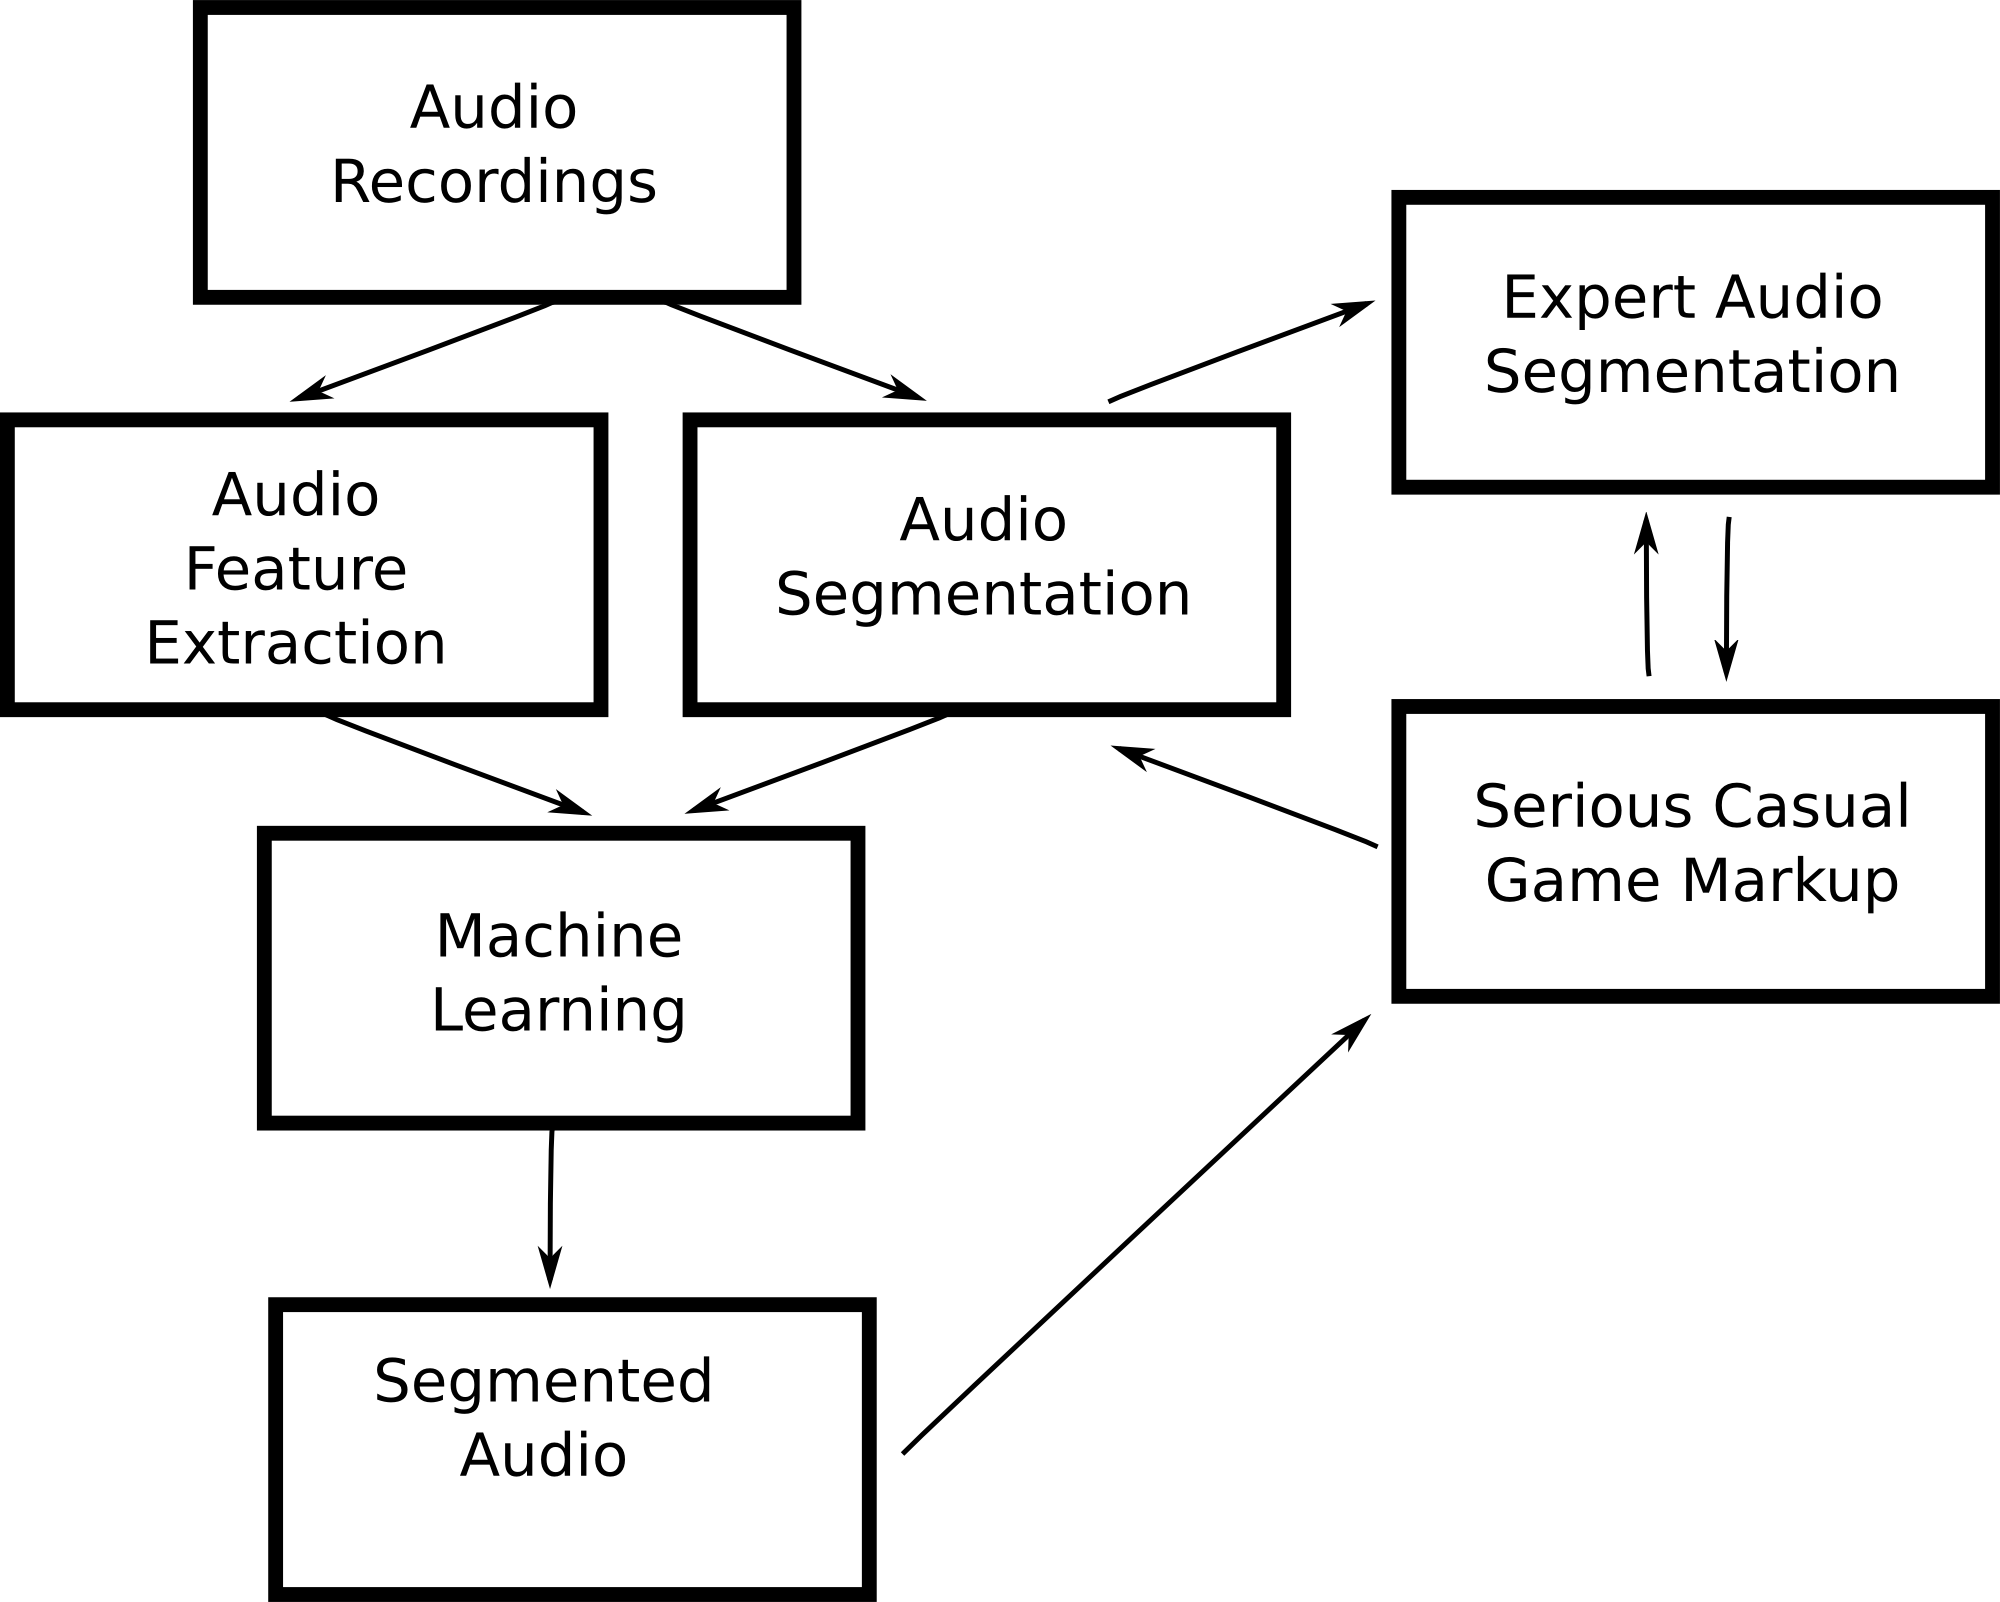
\includegraphics[width=80mm]{chapter_software_and_systems/systemDiagram}
\caption{System Diagram} 
\label{fig:systemDiagram} 
\end{figure} 

In order to do this, we will compare a number of different solutions
for doing distributed audio feature extraction and Machine Learning
and will compare not only their performance in classifying audio, but
also our experience with using these tools.

For my evaluation, we will generate two different types of results.
The first type will be the output of the audio feature extraction and
Machine Learning task. For this task, we will look at the distribution
of orca vocalizations in the dataset, and will train Machine Learning
classifiers that can distinguish regions of the Orchive that have
individual orca vocalizations.


\section{Solution}

In order to analyze the audio in large online archives efficiently, a
scenario involving distributed computing must be used.  There are many
different types of systems that perform Machine Learning and many of
these can distribute their work to different machines.  Some of these
systems are better suited for this task than others, and in this paper
we investigate a few combinations of these tools.

One of the possible solutions to the problem of the segmentation of
audio into orca vocalizations and other sounds is to use a Machine
Learning supervised classifier system.  These systems require hand
labelled training data, in our particular case, audio would be
labelled as either orca or background.  This training data is then
used to train a classifier system that can classify future instances
based on features of the training data.  There are a wide variety of
classification algorithms that are commonly used, some of the most
popular are Support Vector Machines (SVMs), Neural Nets, Decision
Trees and Logistic Regression.  In our past work we have found good
success in using SVMs, and have shown that SVMs typically outperform
many other Machine Learning algorithms.  However, there is current
work in this area showing the benefits of many alternate algorithms
for different problem domains.

There are two steps to the problem of the classification of audio
signals.  The first is that of audio feature extraction, and the
second is that of classification with Machine Learning systems.  Sound
is a pressure wave in the air, and the variations in pressure over
time can be stored in a computer as real number values.  This raw
waveform data contains all the information of the signal, but because
of it's extremely high dimensionality, is difficult to analyze with
machine learning systems.  To take this raw data and to put it in a
form more conducive for analysis, we generate a large number of higher
level features, including spectral features \cite{marsyas}, pitch
information \cite{cheveigne02}, chromatic scale information
\cite{marsyas} and other features based on models of the auditory
cortex \cite{lyon82}.  One can also model the statistical behaviour of
these properties as they change over time, an avenue that has been
shown to be fruitful \cite{marsyas}.  In our system we investigated
the use of a number of audio features, the results of which are
discussed in the Evaluation section, but in summary we found that
using all the standard audio features was most useful, however using
pitch information degraded performance of the classifier.  This is a
surprising result and one that we are investigating further.

The second step is to take these audio features, train and test a
Machine Learning classifer on them, and then run this Machine Learning
classifier over all the data.  In many cases it is beneficial to
pre-calculate the audio features for the data, as once as good
parameters can be determined for the audio feature extraction engine,
such as the window size, hop size for the spectrum calculation and the
memory size for the windowed statistical calculations, these features
can be saved and reused in multiple Machine Learning experiments with
different parameters.  One example of this is the recent release of
the Echonest audio features for the Million Song Dataset
\cite{bertinmahieux11}.  This collection of audio features for one
million popular songs took a considerable amount of time to process,
and one approach is to save these audio features and running different
machine learning algorithms or different parameter sets of these
algorithms on them.  Another point that should be made here is that
the form of the features that are extracted in this step can have a
direct relation to the performance of the subsequent Machine Learning
step.  Different algorithms perform better with different forms of
data, and matching the right features to the right algorithm is both
an art and a science.

It should be noted that both of these steps, the audio feature
extraction and the Machine Learning could be carried out in the same
executable.  There are a number of advantages to this as well as some
disadvantages.  One major advantage is that the intermediate audio
feature data does not have to be saved on disk.  This intermediate
data can be very large in size, and can be many times larger in size
than the original audio data, depending on the type of compression
used for the original audio.  In many cases in the real world, it is
less expensive to just recalculate the audio features each time that a
new Machine Learning run is carried out rather than saving them on
disk.  This also can help to overcome any versioning problems, where
different versions of audio features are combined together in the
training, testing or predicting stages.  It will be a balance between
these two poles for production systems to manage.

For this work, Marsyas was used for doing Audio Feature Extraction.
There are other Music Information Retrieval toolkits for extracting
audio features, but the audio features output by Marsyas are typically
amongst the most robust and high performing in the literature
\cite{marsyas}.  We have implemented this feature extraction using
native filesystem operations loading data off of NFS or a local disk
depending on the cluster situation.

For the Machine Learning half of the project, a variety of Machine
Learning systems and algorithms were used and comparison of them in is
provided in the evaluation section.  Results have been produced for a
Logistic Regression system using a Stochastic Gradient Descent
algorithm on Mahout, a distributed Machine Learning system implemented
as a Java library on top of Hadoop, an open source clone of the Google
File System (GFS) and Google MapReduce system.  These results are
compared to a Logistic Regression system using a quasi Newton solver
as implemented in Weka, a popular system for Machine Learning and show
timing and classification results of this system run as a grid style
parallel job on Westgrid.  These results for Logistic Regression are
then compared to three different implementations of a Support Vector
Machine (SVM) classifier.  The first of these is simply the SVM mode
in Weka but run in a grid-style distributed manner.  The second of
these is a parallel version of the SVM algorithm, PSVM
\cite{chang07psvm}.  The third of these is a hybrid audio feature
extraction and SVM developed in the Marsyas framework.  These three
different systems will be compared and contrasted in the Evaluation
section.

I propose to use the Westgrid system for running the huge audio
feature extraction task. This uses a very simple queuing system known
as Torque, which is the latest evolution of the ancient PBS (Parallel
Batch System) parallel job distribution system. PBS allows scientific
users to schedule large jobs to run on computers, and performs well
for certain scientific tasks where a single, usually large, program is
run on a variety of different datasets, and the results are then saved
to disk and later analyzed by a scientist. This type of computing was
traditionally known as Grid Computing.  While this system has certain
benefits for running specific scientific tasks, for other tasks, the
methodology of having separate computers running mostly independently,
and all coordination of tasks being the responsibility of the
programmer with an tool such as MPI quickly becomes difficult. The
MapReduce paradigm helps in the coordination of large parallel tasks,
and the Hadoop system allows programmers to efficiently write
distributed programs that run on huge numbers of computers and allows
for failures of individual computers. In this project we will use the
Mahout Machine Learning framework on top of a Hadoop installation to
process the audio feature vectors output by Marsyas and to gain
insights into the vocalization data in the Orchive. The primary task I
will investigate in this project will be identifying regions of the
Orchive with distinct orca vocalizations that are nearby to
hydrophones and isolated from other orca vocalizations.

Mahout is a Machine Learning framework that interacts closely with
Hadoop to both store the data and also run the Machine Learning
algorithms.  Hadoop is an open source port of the GFS
\cite{ghemawat03} and MapReduce \cite{dean08} infrastructure and
allows users to run large jobs that follow the map reduce paradigm.
In this scheme, a parallel job is split into two phases, a map phase
and a reduce phase.  In the map phase, key value pairs are generated
by some given algorithm from an input file, this same process occurs
in parallel on many other nodes, and the data that is used by a given
map is determined by the locality of data on that node.  These key
value pairs are then sorted and shuffled to a set of reduce nodes,
which take the collections of key value pairs and do an operation on
them that in some way combines, or reduces, the data.  These map and
reduce functions can be thought of as similar to the map and reduce
functions in functional programming, however, it should be noted that
this is a loose similarity due to the lack of higher order functions
in the current MapReduce implementation.  Many algorithms have been
ported to use this MapReduce type system, some of the most natural are
those that process large collections of text for building inverted
indexes or other tasks for searches, which is not surprising noting
the provenance of the MapReduce algorithm.  For other tasks, such as
those common in audio feature extraction, the reduce phase is simply
an identity reduce, where the map outputs are copied verbatim to the
reduce outputs.  It is easier and more natural to make some algorithms
more efficient in a MapReduce context than others.

The Mahout Machine Learning framework has implemented many different
Machine Learning algorithms in it's framework, including clustering,
recommendation and classification algorithms.  In our current work we
are more interested in classification than either recommendation or
clustering, and Mahout boasts support for the following classification
algorithms: Logistic Regression (SGD), Bayesian, Support Vector
Machines (SVM), Perceptron and Winnow, Neural Network, Random Forests,
Restricted Boltzmann Machines, Online Passive Aggressive, Boosting and
Hidden Markov Models.  However, after investigation, it appears most
of these algorithms are in a definite alpha state, and require
patching of the main source tree with external files.  The two most
well supported classification algorithms in Mahout are the Logistic
Regression classifier, using a Stochastic Gradient Descent (SGD)
engine, and a Naive Bayesian classifier.  Upon extensive
investigation, the Bayesian classifier makes many internal assumptions
of the input being of large bodies of written text and was not
suitable for our use case.  However, the Logistic Regression
classifier was well suited to our data and performed well in our
tests.

One advantage of using the Mahout Machine Learning framework was that
it stored its input and output data on HDFS, the Hadoop Distributed
Filesystem.  When working with the huge amounts of data that are
generated by audio feature extraction and Machine Learning
experiments, managing and transferring experimental results from the
grid servers to the production web servers is often a time consuming
and error prone procedure.  After our experience with Hadoop, we have
integrated it into web application and use the WebHDFS system to serve
all experimental results to users.  These users interact with a web
application that displays some data obtained from the production web
server but also displays the results of experiments as data served
live from a WebHDFS system that is being populated by the experimental
results from live requests from scientists.



%%%%%%%%%%%%%%%%%%%%%%%%%%%%%%%%%%%%%%%%%%%%%%%%%%%%%%%%%%%%%%%%%%%%%%%%%%%%%%%%
%%%%%%%%%%%%%%%%%%%%%%%%%%%%%%%%%%%%%%%%%%%%%%%%%%%%%%%%%%%%%%%%%%%%%%%%%%%%%%%%


\section{Auditory Sparse Coding}

\section{Summary}

% REWRITE
The concept of sparsity has attracted considerable interest in the
field of machine learning in the past few years.  Sparse feature
vectors contain mostly values of zero and one or a few non-zero
values.  Although these feature vectors can be classified by
traditional machine learning algorithms, such as SVM, there are various
recently-developed algorithms that explicitly take advantage of
the sparse nature of the data, leading to massive speedups in time, as
well as improved performance.  Some fields that have benefited from
the use of sparse algorithms are finance, bioinformatics, text mining
\cite{balakrishnan2008}, and image classification \cite{chechik2010}.
Because of their speed, these algorithms perform well on very large
collections of data \cite{bottou2007}; large collections are becoming 
increasingly relevant given the huge amounts of data collected and warehoused 
by Internet businesses.
% REWRITE

% REWRITE
In this chapter, we discuss the application of sparse feature vectors
in the field of audio analysis, and specifically their use in conjunction with 
preprocessing systems that model the human auditory system. We present early
results that demonstrate the applicability of the combination of 
auditory-based processing and sparse coding to content-based audio analysis 
tasks.
% REWRITE

% REWRITE
We present results from two different experiments: a search task in which 
ranked lists of sound effects are retrieved from text queries, and a music 
information retrieval (MIR) task dealing with the classification of music into 
genres.
% REWRITE

\section{Introduction}

% REWRITE
Traditional approaches to audio analysis problems typically employ a 
short-window fast Fourier transform (FFT) as the first stage of the processing 
pipeline. In such systems a short, perhaps 25ms, segment of audio is taken 
from the input signal and windowed in some way, then the FFT of that segment 
is taken. The window is then shifted a little, by perhaps 10ms, and the 
process is repeated. This technique yields a two-dimensional spectrogram of 
the original audio, with the frequency axis of the FFT as one dimension, and 
time (quantized by the step-size of the window) as the other dimension.
% REWRITE

% REWRITE
While the spectrogram is easy to compute, and a standard engineering tool, it 
bears little resemblance to the early stages of the processing pipeline in the 
human auditory system. The mammalian cochlea can be viewed as a bank of tuned 
filters the output of which is a set of band-pass filtered versions of the 
input signal that are continuous in time. Because of this property, 
fine-timing information is preserved in the output of cochlea, whereas in the 
spectrogram described above, there is no fine-timing information available 
below the 10ms hop-size of the windowing function.
% REWRITE

% REWRITE
This fine-timing information from the cochlea can be made use of in later 
stages of processing to yield a three-dimensional representation of audio, the 
stabilized auditory image (SAI)\cite{patterson2000}, which is a movie-like representation of sound which has a dimension of 
`time-interval' in addition to the standard dimensions of time and frequency 
in the spectrogram. The periodicity of the waveform gives rise to a vertical 
banding structure in this time interval dimension, which provides information 
about the sound which is complementary to that available in the frequency 
dimension. A single example frame of a stabilized auditory image is shown in Figure~\ref{fig:sai}.
% REWRITE

% REWRITE
While we believe that such a representation should be useful for audio 
analysis tasks, it does come at a cost. The data rate of the SAI is many times 
that of the original input audio, and as such some form of dimensionality 
reduction is required in order to create features at a suitable data rate for 
use in a recognition system. One approach to this problem is to move from a 
the dense representation of the SAI to a sparse representation, in which the 
overall dimensionality of the features is high, but only a limit number of the 
dimensions are nonzero at any time.
% REWRITE

% REWRITE
In recent years, machine learning algorithms that utilize the properties of 
sparsity have begun to attract more attention and have been shown to 
outperform approaches that use dense feature vectors.  One such algorithm is 
the passive-aggressive model for image retrieval (PAMIR), a machine
learning algorithm that learns a ranking function from the input data,
that is, it takes an input set of documents and orders them based on
their relevance to a query. PAMIR was originally developed as a machine
vision method and has demonstrated excellent results in this field.
% REWRITE

% REWRITE
There is also growing evidence that in the human nervous
system sensory inputs are coded in a sparse manner; that is, only
small numbers of neurons are active at a given time
\cite{olshausen2004}.  Therefore, when modeling the human auditory
system, it may be advantageous to investigate this property of
sparseness in relation to the mappings that are being developed. The
nervous systems of animals have evolved over millions of years to be
highly efficient in terms of energy consumption and computation. 
Looking into the way sound signals are handled by the auditory
system could give us insights into how to make our algorithms more
efficient and better model the human auditory system.
% REWRITE

% REWRITE
One advantage of using sparse vectors is that such coding allows very fast
computation of similarity, with a trainable similarity measure 
\cite{chechik2010}. The efficiency results from storing, accessing, and doing 
arithmetic operations on only the non-zero elements of the vectors.   
In one study that examined the performance of sparse
representations in the field of natural language processing, a 20- to
80-fold speedup over LIBSVM was found \cite{haffner2006}.  They
comment that kernel-based methods, like SVM, scale quadratically with
the number of training examples and discuss how sparsity can allow
algorithms to scale linearly based on the number of training examples.
% REWRITE

% REWRITE
In this chapter, we use the stabilized auditory image (SAI) as the basis of a 
sparse feature representation which is then tested in a sound ranking task and 
a music information retrieval task. In the sound raking task, we generate a 
two-dimensional SAI for each time slice, and then sparse-code those images as 
input to PAMIR.  We use the ability of PAMIR to learn representations of 
sparse data in order to learn a model which maps text terms to audio features. 
This PAMIR model can then be used rank a list of unlabeled sound effects 
according to their relevance to some text query. We present results that show 
that in certain tasks our methods can outperform highly tuned FFT based 
approaches. We also use similar sparse-coded SAI features as input to a music 
genre classification system. This system uses an SVM classifier on the sparse
features, and learns text terms associated with music. The system was entered 
into the annual music information retrieval evaluation exchange 
evaluation (MIREX 2010).
% REWRITE

% REWRITE
Results from the sound-effects ranking task show
that sparse auditory-model-based features outperform standard MFCC
features, reaching precision about 73\% for the top-ranked sound,
compared to about 60\% for standard MFCC and 67\% for the best MFCC
variant.  These experiments involved ranking sounds in response to
text queries through a scalable online machine learning approach to
ranking.
% REWRITE

\subsection{The stabilized auditory image}

% REWRITE
In our system we have taken inspiration from the human auditory system
in order to come up with a rich set of audio features that are
intended to more closely model the audio features that we use to
listen and process music.  
% REWRITE

% REWRITE
Such fine timing relations are discarded by traditional
spectral techniques.  A motivation for using auditory models is that
the auditory system is very effective at identifying many sounds.
This capability may be partially attributed to acoustic features that are
extracted at the early stages of auditory processing.  We feel that
there is a need to develop a representation of sounds that captures
the full range of auditory features that humans use to discriminate
and identify different sounds, so that machines have a chance to do so
as well.  
% REWRITE

% REWRITE
This SAI representation generates a 2D image from each section of
waveform from an audio file.  We then reduce each image in several
steps: first cutting the image into overlapping boxes converted to
fixed resolution per box; second, finding row and column sums of these
boxes and concatenating those into a vector; and finally vector
quantizing the resulting medium-dimensionality vector, using a
separate codebook for each box position.  The VQ codeword index is a
representation of a 1-of-N sparse code for each box, and the
concatenation of all of those sparse vectors, for all the box
positions, makes the sparse code for the SAI image.  The resulting
sparse code is accumulated across the audio file, and this histogram
(count of number of occurrences of each codeword) is then used as
input to an SVM \cite{yh05} classifier\cite{chapelle2006}.  This
approach is similar to that of the ``bag of words'' concept,
originally from natural language processing, but used heavily in
computer vision applications as ``bag of visual words''; here we have
a ``bag of auditory words'', each ``word'' being an abstract feature
corresponding to a VQ codeword.  The bag representation is a list of
occurrence counts, usually sparse.
% REWRITE



\section{Algorithm}

% REWRITE
In our experiments, we generate a stream of SAIs using a series of modules
that process an incoming audio stream through the various stages of the 
auditory model. The first module filters the audio using the
pole--zero filter cascade (PZFC) \cite{lyon10}, then subsequent modules find 
strobe points in this audio, and generate a stream of SAIs at a rate of 50 per 
second. The SAIs are then cut into boxes and are transformed into a high 
dimensional dense feature vector \cite{rehn2009} which is vector quantized to 
give a high dimensional sparse feature vector. This sparse vector is then used 
as input to a machine learning system which performs either ranking or 
classification. This whole process is shown in diagrammatic form in Figure 
~\ref{fig:flowchart}
% REWRITE


\subsection{Pole--Zero Filter Cascade}
% REWRITE
We first process the audio with the pole--zero filter cascade (PZFC)
\cite{lyon10}, a model inspired by the dynamics of the human
cochlea. The PZFC is a cascade of a large number of simple filters with an 
output tap after each stage. The effect of this filter cascade is to transform 
an incoming audio signal into a set of band-pass filtered versions of the 
signal. In our case we used a cascade with 95 stages, leading to 95 output 
channels. Each output channel is half-wave rectified to simulate the output of 
the inner hair cells along the length of the cochlea. The PZFC also includes 
an automatic gain control (AGC) system that mimics the effect of the dynamic 
compression mechanisms seen in the cochlea. A smoothing network, fed from the 
output of each channel, dynamically modifies the characteristics of the 
individual filter stages. The AGC can respond to changes in the 
output on the timescale of milliseconds, leading to very fast-acting 
compression. One way of viewing this 
filter cascade is that its outputs are an approximation of the instantaneous 
neuronal firing rate as a function of cochlear place,  modeling both the 
frequency filtering and the automatic gain control characteristics of the 
human cochlea \cite{lyon1990}. The PZFC parameters used for 
the sound-effects ranking task are described in \cite{lyon10}. We did not do 
any further tuning of this system to the problems of genre, mood or song 
classification; this would be a fruitful area of further research.
% REWRITE


\subsection{Image Stabilization}

% REWRITE
The output of the PZFC filterbank is then subjected to a process of
strobe finding where large peaks in the PZFC signal are found.  The
temporal locations of these peaks are then used to initiate a process
of temporal integration whereby the stabilized auditory image is
generated.  These strobe points ``stabilize'' the signal in a manner
analogous to the trigger mechanism in an oscilloscope.  When these
strobe points are found, a modified form of autocorrelation, known as
strobed temporal integration, which is like a sparse version of
autocorrelation where only the strobe points are correlated against
the signal. Strobed temporal integration has the advantage of being
considerably less computationally expensive than full autocorrelation.
% REWRITE

\subsection{Box Cutting}

% REWRITE
We then divide each image into a number of overlapping boxes using the
same process described in \cite{lyon10}.  We start with rectangles
of size 16 lags by 32 frequency channels, and cover the SAI with these 
rectangles, with overlap.  Each of
these rectangles is added to the set of rectangles to be used for
vector quantization.  We then successively double the height of the rectangle 
up to the largest size that fits in an SAI frame, but always reducing the 
contents of each box back to 16 by 32 values.  Each of these doublings
is added to the set of rectangles.  We then double the width of each
rectangle up to the width of the SAI frame and add these rectangles to
the SAI frame.  The output of this step is a set of 44 overlapping
rectangles. The process of box-cutting is shown in Figure 
~\ref{fig:boxcutting}.
% REWRITE

% REWRITE
In order to reduce the dimensionality of these rectangles, we then
take their row and column marginals and join them together into a
single vector.
% REWRITE

\subsection{Vector Quantization}

% REWRITE
The resulting dense vectors from all the boxes of a frame are then converted 
to a sparse representation by vector quantization.  
% REWRITE

% REWRITE
We first preprocessed a collection of 1000 music files from 10 genres
using a PZFC filterbank followed by strobed temporal integration to
yield a set of SAI frames for each file .  We then take this set of
SAI and apply the box-cutting technique described above. The followed
by the calculation of row and column marginals.  These vectors are
then used to train dictionaries of 200 entries, representing abstract
``auditory words'', for each box position, using a k-means algorithm.
% REWRITE

% REWRITE
This process requires the processing of large amounts of data, just to
train the VQ codebooks on a training corpus.
% REWRITE

% REWRITE
The resulting dictionaries for all boxes are then used in the MIREX
experiment to convert the dense features from the box cutting step on
the test corpus songs into a set of sparse features where each box was
represented by a vector of 200 elements with only one element being
non-zero.  The sparse vectors for each box were then concatenated, and
these long spare vectors are histogrammed over the entire audio file
to produce a sparse feature vector for each song or sound effect.
This operation of constructing a sparse bag of auditory words was done
for both the training and testing corpora.
% REWRITE

\subsection{Machine Learning}

% REWRITE
For this system, we used the support vector machine learning system
from libSVM which is included in the Marsyas\cite{marsyas} framework.
Standard Marsyas SVM parameters were used in order to classify the
sparse bag of auditory words representation of each song.  It should
be noted that SVM is not the ideal algorithm for doing classification
on such a sparse representation, and if time permitted, we would have
instead used the PAMIR machine learning algorithm as described in
\cite{lyon10}.  This algorithm has been shown to outperform SVM on
ranking tasks, both in terms of execution speed and quality of
results.
% REWRITE

\section{Experiments}


\subsection{Sound Ranking}

% REWRITE
We performed an experiment in which we examined a quantitative ranking
task over a diverse set of audio files using tags associated with the
audio files.
% REWRITE

% REWRITE
For this experiment, we collected a dataset of 8638 sound effects,
which came from multiple places.  3855 of the sound files were from
commercially available sound effect libraries, of these 1455 were from
the BBC sound effects library.  The other 4783 audio files were
collected from a variety of sources on the internet, including
findsounds.com, partnersinrhyme.com, acoustica.com, ilovewaves.com,
simplythebest.net, wav-sounds.com, wav-source.com and wavlist.com.
% REWRITE

% REWRITE
We then manually annotated this dataset of sound effects with a small
number of tags for each file.  Some of the files were already assigned
tags and for these, we combined our tags with this previously existing
tag information.  In addition, we added higher level tags to each
file, for example, files with the tags ``cat'', ``dog'' and ``monkey''
were also given the tags ``mammal'' and ``animal''.  We found that the
addition of these higher level tags assist retrieval by inducing
structure over the label space.  All the terms in our database were
stemmed, and we used the Porter stemmer for English, which left a
total of 3268 unique tags for an average of 3.2 tags per sound file.
% REWRITE

% REWRITE
In order to estimate the performance of the learned ranker, we used a
standard three-fold cross-validation experimental setup.  In this
scheme, two thirds of the data is used for training and one third is
used for testing; this process is then repeated for all three splits
of the data and results of the three are averaged.  We removed any
queries that had fewer than 5 documents in either the training set or
the test set, and if the corresponding documents had no other tags,
these documents were removed as well.
% REWRITE

% REWRITE
To determine the values of the hyperparameters for PAMIR we performed a
second level of cross-validation where we iterated over values for the
aggressiveness parameter C and the number of training iterations.  We
found that in general system performance was good for moderate values
of C and that lower values of C required a longer training time.  For
the agressiveness parameter, we selected a value of C=0.1, a value
which was also found to be optimal in other research
\cite{grangier2008}.  For the number of iterations, we chose 10M, and
found that in our experience, the system was not very sensitive to the
exact value of these parameters.
% REWRITE

% REWRITE
We evaluated our learned model by looking at the precision within the
top k audio files from the test set as ranked by each query.
Precision at top k is a commonly used measure in retrieval tasks such as these
and measures the fraction of positive results within the top k results from a
query.
% REWRITE

% REWRITE
The stabilized auditory image generation process has a number of
parameters which can be adjusted including the parameters of the PZFC
filter and the size of rectangles that the SAI is cut into for
subsequent vector quantization.  We created a default set of
parameters and then varied these parameters in our experiments.  The
default SAI box-cutting was performed with 16 lags and 32 channels,
which gave a total of 49 rectangles.  These rectangles were then
reduced to their marginal values which gives a 48 dimension vector,
and a codebook of size 256 was used for each box, giving a total of 49
x 256 = 12544 feature dimensions.  Starting from these, we then made
systematic variations to a number of different parameters and measured
their effect on precision of retrieval.  For
the box-cutting step, we adjusted various parameters including the
smallest sized rectangle, and the maximum number of rectangles used
for segmentation.  We also varied the codebook sizes that we used in
the sparse coding step.
% REWRITE

% REWRITE
In order to evaluate our method, we compared it with results obtained
using a very common feature extraction method for audio analysis, MFCCs
(mel-frequency cepstral coefficients).  In order to compare this type
of feature extraction with our own, we turned these MFCC coefficients
into a sparse code.  These MFCC coefficients were calculated with a
Hamming window with initial parameters based on a setting optimized
for speech.  We then changed various parameters of the MFCC algorithm,
including the number of cepstral coefficients (13 for speech), the
length of each frame (25ms for speech), and the number of codebooks
that were used to sparsify the dense MFCC features for each frame.  We
obtained the best performance with 40 cepstral coefficients, a window
size of 40ms and codebooks of size 5000.
% REWRITE




\section{Audio Feature Extraction}

\subsection{Campana}


% REWRITE
In the paper ``Monitoring and Mining Insect Sounds in Visual
Space''\cite{hao12}, Hao et al. describe a novel method for data
mining large databases of insect sounds.  Their method is completely
automated, and does not require human experts to label data, as is the
case in most other systems of this type.  They perform classification
of sounds based on the spectrogram, a visual representation of a sound
that gives a frequency versus time plot of a sound.  They use a recent
distance measure called the Campana-Keogh (CK) measure to compare the
textures of two images.  
% REWRITE

% REWRITE
The paper first describes the importance of monitoring and measuring
of the sounds of animals and insects.  In the natural habitat, the
sounds of animals can be used to determine how many animals are in a
location and what species these animals are, and can help scientists
measure the biodiversity of a location, and how this biodiversity
changes over time.  There is recent interest in this field of study
\cite{wimmer2010} %% \cite{seuer2008}
as a method for determining the
biodiversity changes in regions over time.  The authors then say that
an automated system for detecting insects would also be useful from a
commercial point of view,
% REWRITE

% REWRITE
The paper then goes on to say that in laboratory settings, it would
also be advantageous to have an automated system that could segment
and classify recordings.  Currently this task often requires
researchers to annotate hundreds of recordings by hand, which is a
very time intensive task.  As a scientist who has done many hours of
hand annotating of large sound archives, I can attest to the
difficulty and time-consuming nature of this task.
% REWRITE

% REWRITE
The authors then say that there are many problems with current methods
of detecting, segmenting and classifying the sounds and vocalizations
of animals.  Current methods require researchers to manually annotate
recordings and to generate a large corpus of data to be used by
classification algorithms.  These algorithms often have a large number
of tunable parameters, some of which can be automatically determined
from the large amount of training data, and some which have to be
manually explored by the researchers.  In addition, many of these
algorithms are computationally expensive and cannot be deployed in the
field.  I have found these facts to be true in my own research, and I
appreciate the fact that the authors spend time discussing the
problems faced by researchers studying bioacoustics.
% REWRITE

% REWRITE
The authors then go on to describe the notation used in their paper.
I found this section challenging to understand at first, and it was
only by repeated readings of this section, and indeed the whole paper,
that I was able to understand what they were trying to convey.  Once I
understood it, I found this section very valuable, but it would have
been useful if they described how each of these notations fit into the
paper as a whole.
% REWRITE

% REWRITE
In this section, they first define a sound sequence as a continuous
sequence of real valued data.  They then go on to define a spectrogram
as a visual spectral representation of an acoustic signal.  They
define a sliding window as a local subsection of a sound sequence, and
define a subsequence and a way to measure distances between
subsequences.
% REWRITE

% REWRITE
They then move on to more interesting definitions, first of the
entropy of a sound sequence dataset:
% REWRITE

% REWRITE
	\[ E(D) = -p(X)log(p(X)) - p(Y)log(p(Y)) \]
% REWRITE

% REWRITE
The information gain for a given splitting strategy is then defined as
% REWRITE

	\[ Gain = E(D) - E'(D) \]

% REWRITE
Where $E(D)$ and $E'(D)$ are the entropy before and after $D$ is
partitioned into $D_1$ and $D_2$.
% REWRITE

	\[ E(D) = f(D_1)E(D_1) + f(D_2)E(D_2) \] 

% REWRITE
Where $f(D_1)$ and $f(D_2)$ are the fraction of the objects that are
in $D_1$ and $D_2$, respectively.
% REWRITE

% REWRITE
They will use these definitions later in the paper to help speed up
the time used by their brute force algorithm.  I find this one of the
most interesting parts of this paper, the use of information entropy
and information gain to speed up their algorithm, which makes this
algorithm practical to use on large datasets.  Without it, the CK
measure on its own would be very expensive to run on all audio frames
in a large data mining experiment.
% REWRITE

% REWRITE
They then point out that given a linear ordering of annotated objects
in $D$, there exist at most $|D|-1$ distinct splitting points that
divide the ordered objects into two distinct sets.  Finally, they
define a sound fingerprint for a species as the subsequence from P
along with its best splitting point that produces the largest
information gain when compared with the non-matching sequences U.
% REWRITE

% REWRITE
They then go on to provide an figure that explains in rough detail
what their distance measure looks like.  This is shown here in Figure
\ref{fig:campana_figure2}.  I found these examples to be unclear at
first, but on deep examination and by staring at it for quite some
time, I figured out what they were trying to say.  In these examples,
they show some sound fingerprints with arrows pointing to a line below
them.
% REWRITE

% REWRITE
The authors then give a very detailed methodology section that
includes not just equations, but also the algorithms that they have
implemented.  I found this section useful and valuable, in that it
gave clear equations for how their method worked, and also presented
an implementation of these equations in an easy to understand series
of algorithms.
% REWRITE

% REWRITE
They first describe the Brute-Force algorithm, which basically just
searches over all possible combinations of subsequences for P and U,
and computes the distance between all these subsequences.  The
equation for this is:
% REWRITE

\[ \sum^{L_{max}}_{l=L_{min}} \sum_{S_i \in { P }} (M_i - l + 1) \]

% REWRITE
While this algorithm guarantees that the best subsequence will be
found, it is quite expensive in terms of computer time, and even for
their toy dataset of 10 sound files of the insect they are looking for
and 10 sound files of other sounds, would take 1,377,800 calls to the
CK distance measure, which is the most time intensive part of the
whole process.
% REWRITE

% REWRITE
To reduce the computation time, they first investigate Admissible
Entropy Pruning, in which they note that they can easily compute the
upper bound of an ordering, and if this upper bound is less than the
best-so-far information gain of any previously determined ordering,
they can abandon the current search and move on to the next candidate.
For their toy problem, this only reduces the total number of
comparisons, but in a data mining context, where huge databases are
searched, they say this could prune the total number of calculations
by 95\%.  This Entropy Pruning algorithm is one of the key insights of
this paper.  Without it, their CK distance measure would likely be too
expensive to use on real datasets, and by using Entropy Pruning, they
are able to speed up their algorithm by a large factor.
% REWRITE

\subsection{SAI}

% REWRITE
The field of Music Information Retrieval (MIR) or Machine Hearing
\cite{marsyas} attempts to teach computers to understand music.  There
are a wide variety of tasks in this field that range from music
playlisting to analyzing Gregorian chants and Bach fugues.  Both in my
group at UVIC and at Google, we are specifically interested in
approaches that take audio as input.  From this audio we calculate a
variety of features, including the low, medium and high frequency
content and how these frequencies evolve over time.  We then use
advanced machine learning algorithms including Support Vector Machines
and Deep Belief Networks \cite{bengio2007}.  
% REWRITE

% REWRITE
Most current approaches in MIR use spectral based approaches that use
the Fast Fourier Algorithm to decompose a signal into a set of
sinusoid's with a specific frequency and phase.  An example spectrogram
of a human voice is shown in Figure \ref{fig:spectrogram}.  These approaches are
computationally efficient and fast, and give us a good understanding
of many features of music.  Using these features, the field of MIR has
had many successes, in the field of genre recognition, for example, we
often can achieve a classification accuracy of 80\%.  In the past 5
years, most of the advances in MIR have come from applying more and
more advanced machine learning algorithms to this problem.  It now
appears that we have reached a plateau where the performance of these
systems is not increasing, and it is felt that by using better audio
features, performance can be again improved.
% REWRITE


% REWRITE
FFT based approaches are fundamentally different from how our ear
actually hears sound.  FFT approaches take a window of data and
decompose this window into different sinusoids with a period and
phase.  The choice of window size involves a tradeoff between time
resolution and frequency resolution, and in order to increase time
resolution, frequency resolution must be decreased.  For certain
sounds produced in music, like those of sustained notes, this model
works well, but for many others, such as drum hits or the pulse
resonance phenomenon found in human voices, this model has
limitations.
% REWRITE

% REWRITE
The models of the human auditory system (Figure \ref{fig:humanear}
developed both by Dick Lyon \cite{slaney93} and other researchers
around the world have a fundamentally different approach in which
audio is filtered by a filterbank cascade that models features of the
human cochlea, the outputs of these filters are then processed by a
mechanism that is modeled on higher levels in the auditory periphery
that take this filterbank audio and generate two dimensional movie
frames that contain both frequency and an autocorrelation axis.  These
frames contain the fine timing information that is utilized by the
human hearing system to separate, localize and identify sounds.
% REWRITE

% REWRITE
We are interested in developing these models to help us with different
machine learning tasks in music, including classifying songs into
genres, finding the most similar songs to a seed song and categorizing
sounds with tags.
% REWRITE

% REWRITE
This model finds trigger points in the input audio signal and
stabilizes the train of peaks from the CARFAC filterbank cascade into
a two dimensional image.  The output of the CARFAC filterbank is shown
in Figure \ref{fig:nap}, in this figure, the vertical axis corresponds
to cochlear place, with points closer to the bottom axis corresponding
to lower frequencies and the horizontal axis corresponding to time.
This plot can also be referred to as a Neural Activity Profile (NAP).
These peaks flow by rapidly, at the rate of pulses from the organism
in question, and in order to view them, one should align subsequent
peaks to each other.  There are many approaches to doing this, and the
approach commonly used is to find trigger points in the audio, that
is, points that correspond to pulses in the output of the vocal tract.
One trigger detection algorithm is shown schematically in Figure
\ref{fig:triggerpoints}.  In this figure the solid black line in the
center corresponds to the audio signal, and the red dots signify
trigger points.  The solid black line at the top of the figure
represents the current threshold value of the algorithm, and when this
threshold crosses the line representing the audio, a new trigger point
is generated.
% REWRITE

In this section, we focus on retrieval rather than classification and
only use the ground truth labels as a way to measure retrieval
effectiveness. We compare different strategies over a large dataset
(185 calls, 4 classes) using well established retrieval effectiveness
measures. To the best of our knowledge this is the first systematic
evaluation of these different design choices.

\subsection{Contour Extraction and Retrieval Strategies}  

The discrete calls of killer whales are pulsed signals in which a tone
(of a certain tonal frequency) is not emitted continuously but in
pulses given by the pulse-repetition rate. Unlike the tonal signals of
many birds and other delphinids, the highest energy is not always
contained in the first or second harmonic
\cite{deecke99_quantifying_orca}. The high levels of background noise
and variety of recording conditions compound the difficulty of
obtaining pulse rate contours. The pulse rate contour is used as the
primary representation for Orca calls because it is more robust as
compared to spectral features to levels of background noise typical in
field recordings.

We have compared three pitch extraction methods for obtaining the
pulse rate contour. The first method ({\bf PRAAT}) is based on
time-domain autocorrelation and is similar to the pitch extraction
algorithm implemented in Praat \cite{boersma93}. It is based on
calculating the time-domain autocorrelation of the signal:

\begin{equation} 
R(\tau) = \frac{1}{N} \sum_{n=0}^{N-1-m} x[n] x[n+m] \;\;\;\; 0 \leq m
< M 
\end{equation} 

The peaks of the autocorrelation function correspond to the lags 
in which the signal is self-similar. The signal is processed in
windows and the autocorrelation of the windowed signal $R_{xw}$ is divided 
by the autocorrelation of the window $R_{w}$ providing better robustness to 
noise and better accuracy. 

\begin{equation}
R_{x}(\tau) = R_{xw}(\tau) / R_{w}(\tau)
\end{equation} 


The second method is based on the {\bf YIN} pitch extraction method.  The YIN method is 
based on the difference function which is similar to the
autocorrelation: 

\begin{equation}
d{t} = \sum_{n=0}^{N-1} (x[n] - x[n+\tau])^{2}
\end{equation} 

The dips in the difference function correspond to periodicities. 
In order to reduce the occurrence of subharmonic errors, YIN employs a
cumulative mean function which de-emphasizes higher period dips 
in the difference function. 

The third method ({\bf SACF}) is based on the multipitch detection algorithm
described by Tolonen and Karjalainen \cite{tolonen00}.  In this algorithm, the
signal is decomposed into two frequency bands (below and above 1000
Hz) and amplitude envelopes are extracted for each frequency band. The
envelope extraction is performed by applying half-wave rectification
and low-pass filtering.  The envelopes are summed and an enhanced
autocorrelation function is computed so that the effect of integer
multiples of the peak frequencies to multiple pitch detection is
reduced.




We explore three retrieval strategies/representations. Statistical
features characterizing the entire pulse rate contour are computed and
each call is characterized by a single vector of features. The
features are normalized by max-min normalization so that they range
from 0 to 1 over the entire dataset. Similarities are then computed by
taking the Euclidean distance in the normalized space. This strategy
is used as reasonable baseline. The features used in this work are the mean, median,
standard deviation, min and max of the pulse rate contour. The second
strategy consists of resampling the pulse rate contour using linear
interpolation to a fixed number of points. This strategy is similar to
the one used in Deecke \cite{deecke99_quantifying_orca}. Essentially
it assumes that the duration of the call does not play a major role in
its characterization and temporal scaling is applied uniformly across
the contour. The third strategy utilizes dynamic time warping to align
the pulse rate contours. The alignment cost is used to measure the
similarity between calls. The two sequences to be matched are arranged
on the sides of a grid. To find the best match between the sequences
we can find a path through the grid that minimizes the total distance
between them. More details can be found in \cite{sakoe78}.


\subsection{SOM}


For creating the visualization layout we utilized the self-organizing
map (SOM) which is a type of neural network used to map a high
dimensional feature space to a lower dimensional representation while
preserving the topology of the high dimensional space. This
facilitates both similarity quantization and visualization
simultaneously. The SOM was first documented in 1982 by T. Kohonen,
and since then, it has been applied to a wide variety of diverse
clustering tasks \cite{kohonen95a}. In our system the SOM is used to
map the audio features (64-dimensions) corresponding to each track
 to two discrete coordinates on a grid.

 The traditional SOM consists of a 2D grid of neural nodes each
 containing a $n$-dimensional vector, $ {\bf x(t)} $ of data. The goal
 of learning in the SOM is to cause different neighbouring parts of
 the network to respond similarly to certain input patterns. The
 network must be fed a large number of example vectors that represent,
 as closely as possible, the kinds of vectors expected during
 mapping. The data associated with each node is initialized to small
 random values before training. During training, a series of
 $n$-dimensional vectors of sample data are added to the map.  The
 ``winning'' node of the map known as the {\it best matching unit}
 (BMU) is found by computing the distance between the added training
 vector and each of the nodes in the SOM. This distance is calculated
 according to some pre-defined distance metric which in our case is
 the standard Euclidean distance on the normalized feature vectors.

Once the winning node has been defined, it and its surrounding nodes
reorganize their vector data to more closely resemble the added
training sample.  The training utilizes competitive learning. The
weights of the BMU and neurons close to it in the SOM lattice are
adjusted towards the input vector. The magnitude of the change
decreases with time and with distance from the BMU. The time-varying
learning rate and neighborhood function allow the SOM to gradually
converge and form clusters

\subsection{PZFC and CARFAC}
The CARFAC model includes a more advanced treatment of the fast acting
compression that the Outer Hair Cells in the cochlea perform to allow
the ear to hear both very loud and very soft sounds, a technique
formally referred to as Automatic Gain Control (AGC).  This model is
more advanced than the PZFC model, and this additional complexity can
be seen in Figure \ref{fig:dspcarfac}.

\begin{figure}[t]
\begin{center}
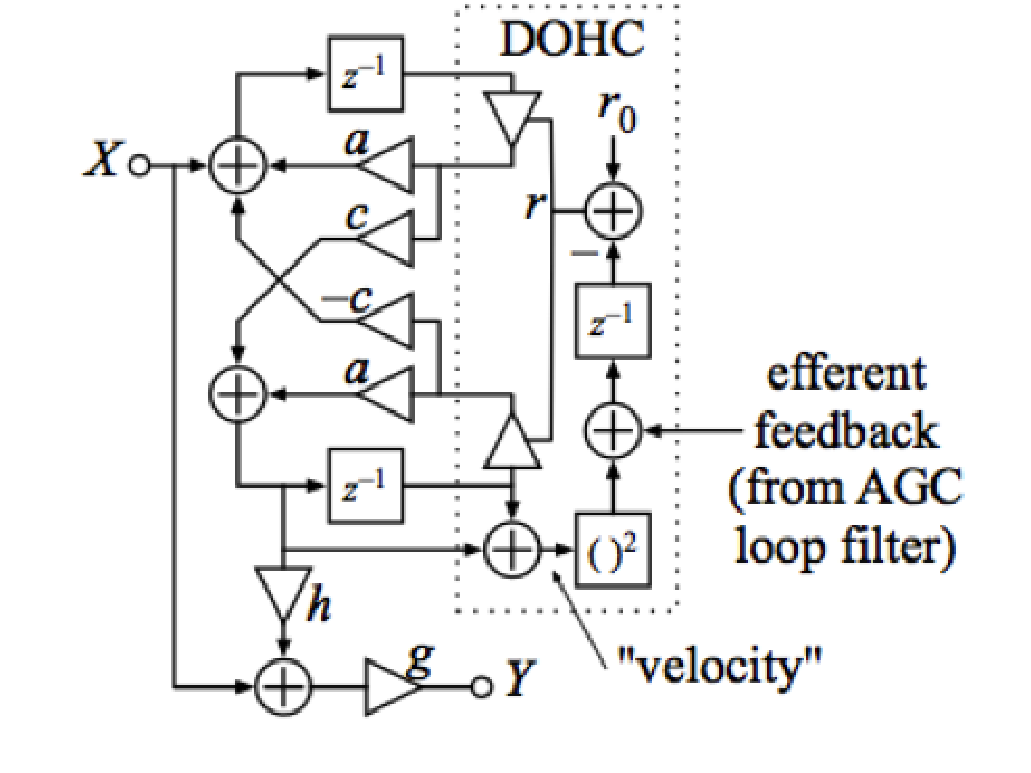
\includegraphics[width=50mm]{images/dspcarfac}
\caption{
The Cascade of Asymmetric Filters and Resonators (CARFAC) model.  This
model is similar to the PZFC model, but includes an Automatic Gain
Control (AGC) stage, that models the action of the Outer Hair Cells in
the human cochlea.} 
\label{fig:dspcarfac} 
\end{center} 
\end{figure} 


The code for the CARFAC model was written in MATLAB, and it was my
task to take this code, port it to C++, verify that it worked
identically to the original code and then to optimize it to run as
quickly as possible.  For this, I used a software development
methodology called Test Driven Development \cite{fraser03} (TDD).  In
TDD, one inverts the normal software development process in that one
first writes the tests, and then the minimum code to make these tests
pass.  This is an ideal development strategy to use in this case,
since we have a working reference implementation of the algorithm in
MATLAB.  Using this strategy, I was able to port this MATLAB code
first to Python and then to C++.  The C++ code was added to the
Marsyas \cite{marsyas} framework and was open-sourced during my time
at Google, and is now available to be used by the community.

The process of porting the CARFAC model was straightforward but time
consuming.  After I had ported this model to C++, we then went back to
MATLAB to develop a model of binaural hearing using the output of the
CARFAC filter cascade.  We used the Stabilized Auditory Image (SAI) model
proposed by Patterson \cite{patterson92}, which works well for the
pulse resonance sounds created by many types of animals, from fish to
insects to the human voice.  In Figure \ref{fig:pulseresonance} the
sounds from various animals are shown, an in each one, the same
phenomenon is seen, where a fast impulse, or pulse is created and is
then resonated through the vocal tract or other sound producing organ
in the creature.

\begin{figure}[t]
\begin{center}
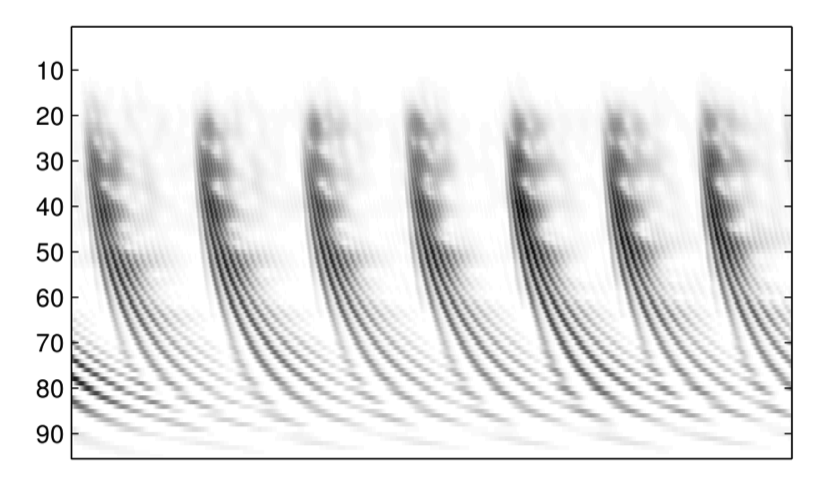
\includegraphics[width=100mm]{images/nap}
\caption{ The Neural Activity Pattern (NAP) of the CARFAC model.  In
  this figure, the vertical axis corresponds to cochlear place, with
  points closer to the bottom axis corresponding to lower frequencies
  and the horizontal axis corresponding to time}
\label{fig:nap} 
\end{center} 
\end{figure} 

\begin{figure}[t]
\begin{center}
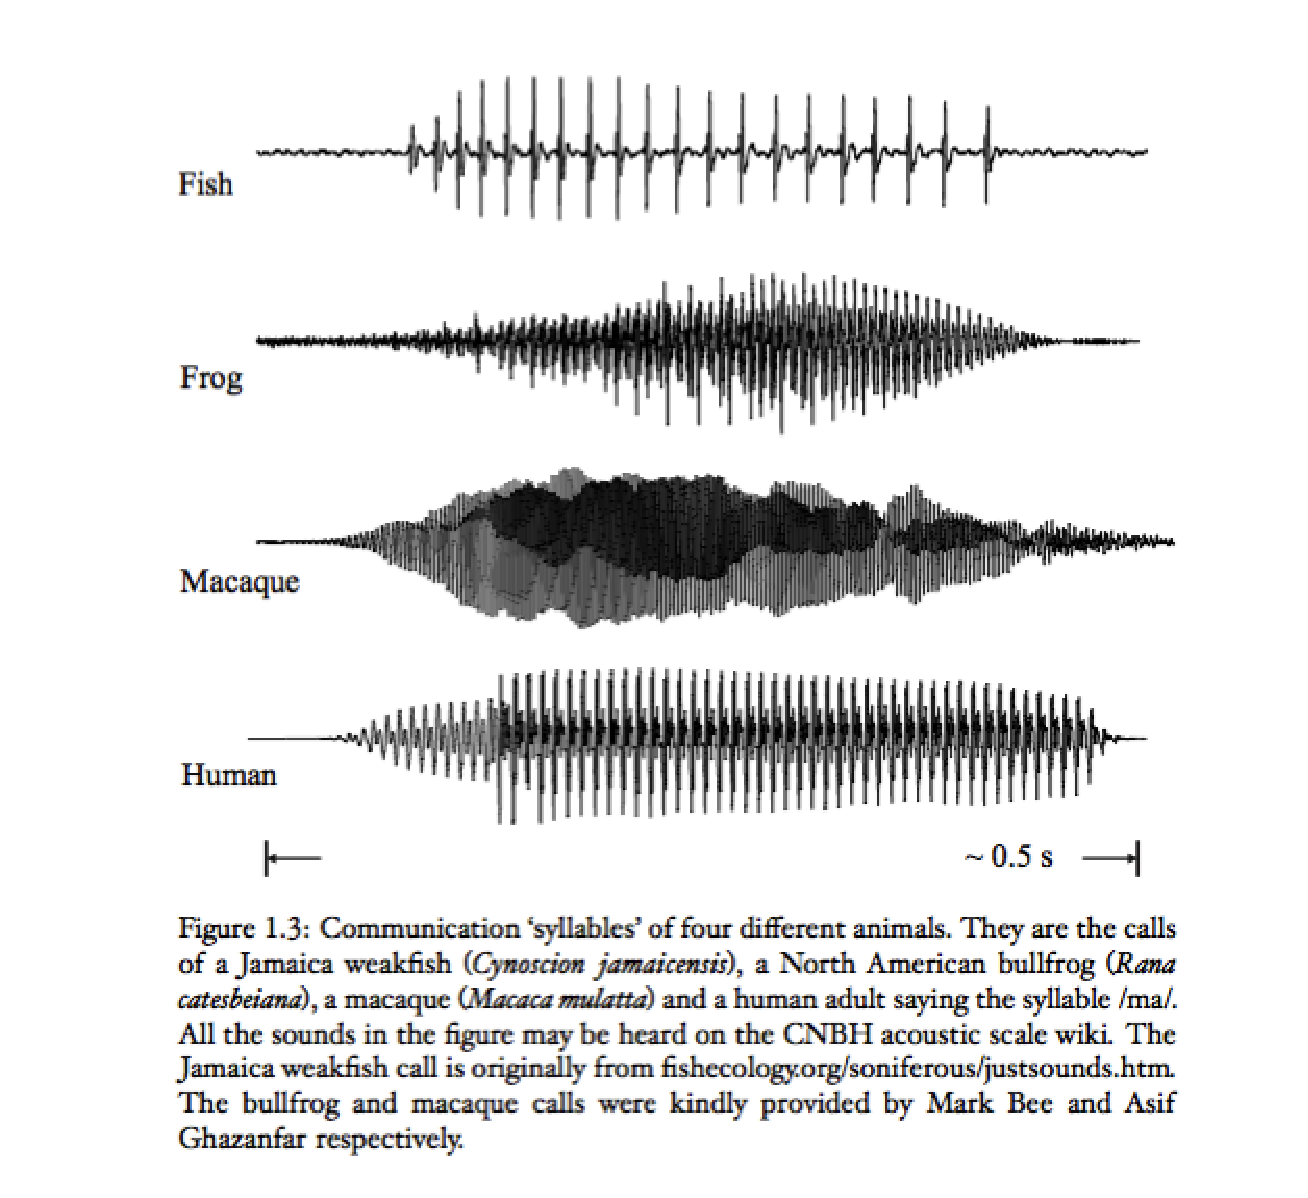
\includegraphics[width=100mm]{images/pulseresonance}
\caption{ A diagram of the waveforms produced by a variety of
  different animals, showing the pulse and resonance structure of
  these vocalizations.  In each, a short pulse is generated which then
  reverberates through the vocal tract or sound producing organ of the
  organism.}
\label{fig:pulseresonance} 
\end{center} 
\end{figure} 

This model finds trigger points in the input audio signal and
stabilizes the train of peaks from the CARFAC filterbank cascade into
a two dimensional image.  The output of the CARFAC filterbank is shown
in Figure \ref{fig:nap}, in this figure, the vertical axis corresponds
to cochlear place, with points closer to the bottom axis corresponding
to lower frequencies and the horizontal axis corresponding to time.
This plot can also be referred to as a Neural Activity Profile (NAP).
These peaks flow by rapidly, at the rate of pulses from the organism
in question, and in order to view them, one should align subsequent
peaks to each other.  There are many approaches to doing this, and the
approach commonly used is to find trigger points in the audio, that
is, points that correspond to pulses in the output of the vocal tract.
One trigger detection algorithm is shown schematically in Figure
\ref{fig:triggerpoints}.  In this figure the solid black line in the
center corresponds to the audio signal, and the red dots signify
trigger points.  The solid black line at the top of the figure
represents the current threshold value of the algorithm, and when this
threshold crosses the line representing the audio, a new trigger point
is generated.

\begin{figure}[t]
\begin{center}
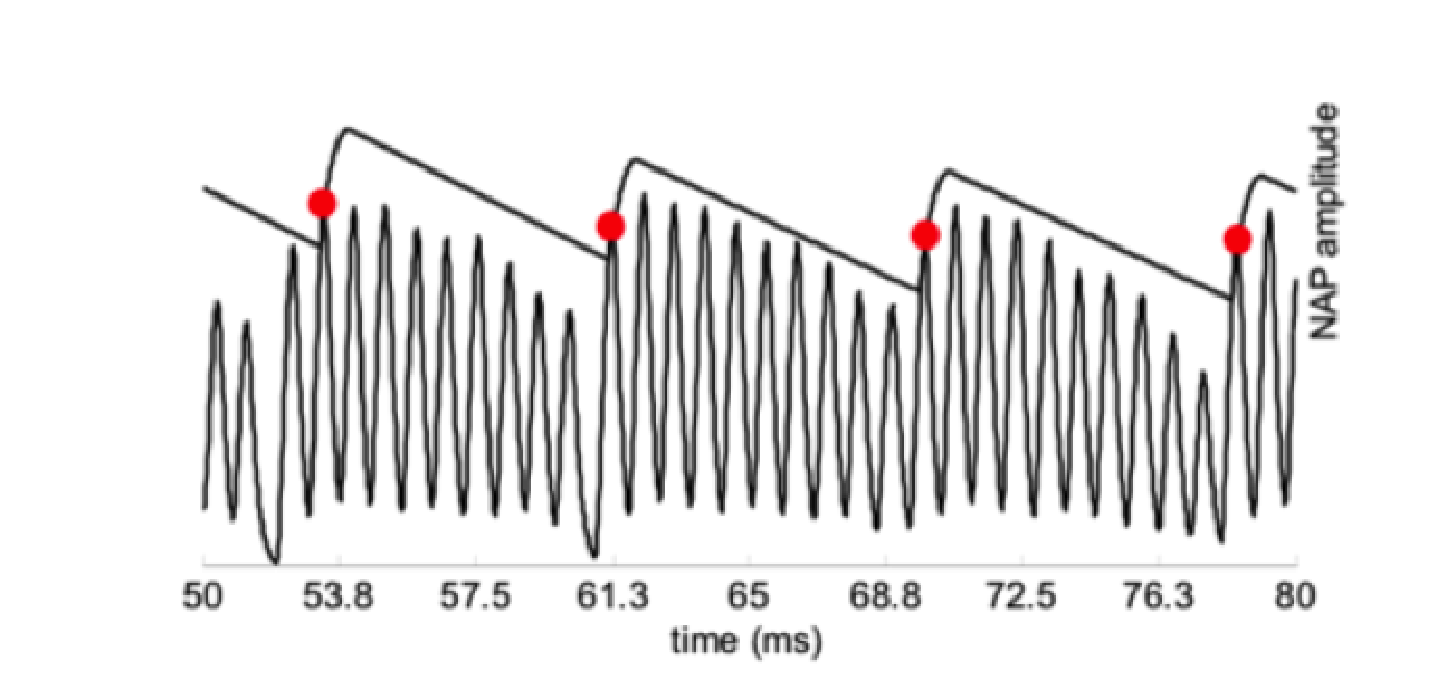
\includegraphics[width=100mm]{images/triggerpoints}
\caption{ In this figure the solid black line in the center
  corresponds to the audio signal, and the red dots signify trigger
  points.  The solid black line at the top of the figure represents
  the current threshold value of the algorithm, and when this
  threshold crosses the line representing the audio, a new trigger
  point is generated.}
\label{fig:triggerpoints} 
\end{center} 
\end{figure} 

\begin{figure}[t]
\begin{center}
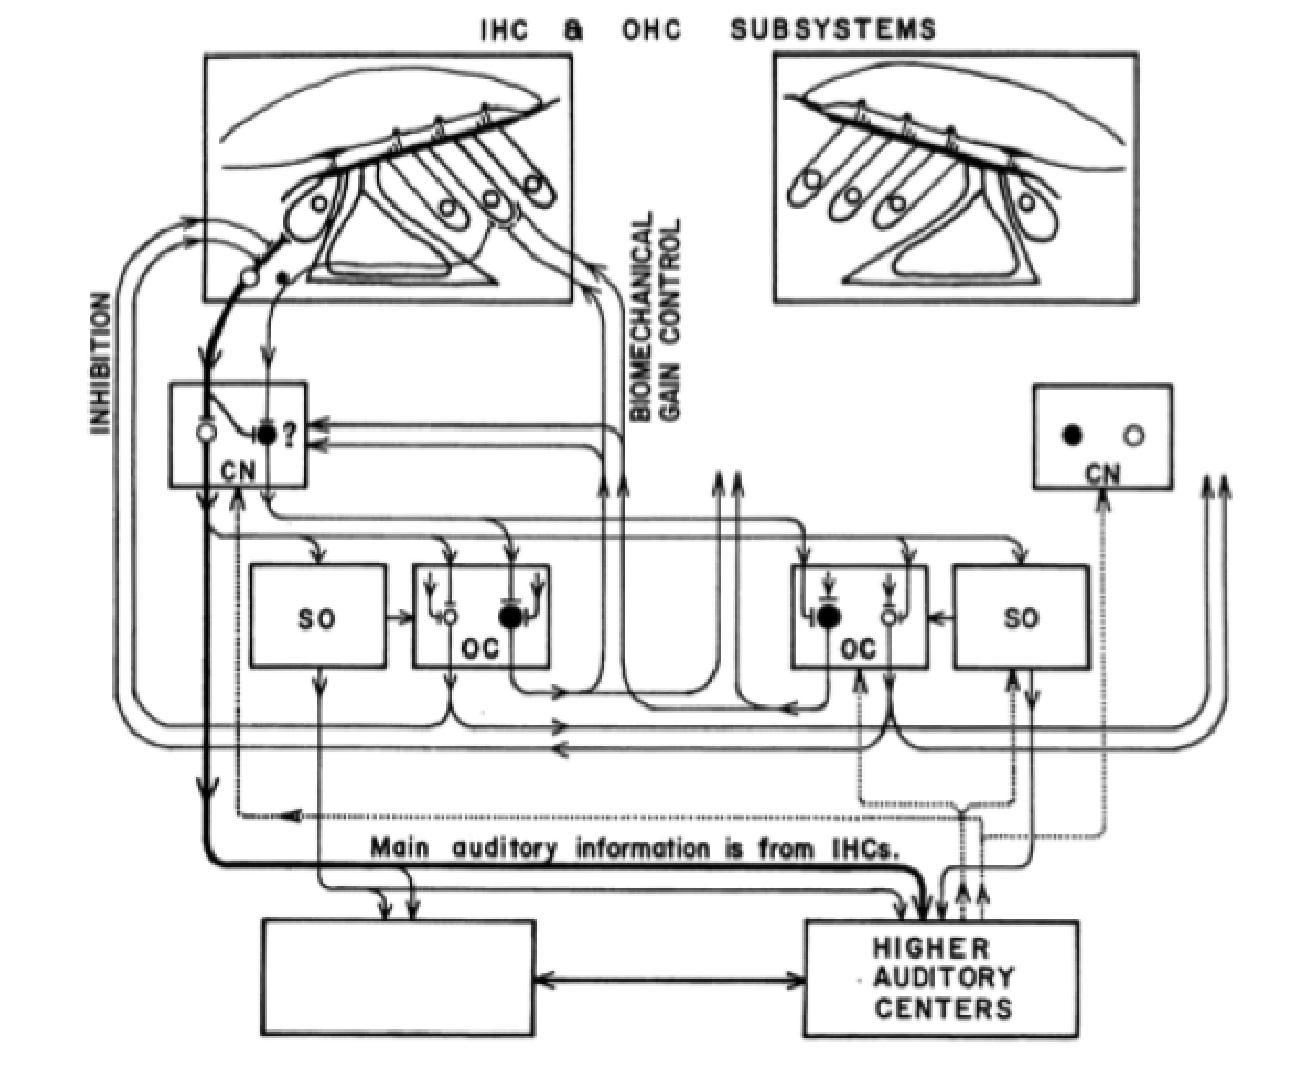
\includegraphics[width=100mm]{images/ihcohc}
\caption{
A schematic view of the connections between the cochlea and the higher
levels of the auditory periphary, including connections between the
olivary complexes to each other and back to their respective cochleas.} 
\label{fig:ihcohc} 
\end{center} 
\end{figure} 


\section{Orchive}

The goal of the Orchive project is to digitize acoustic data that have
been collected over a period of 36 years using a variety of analog
media at the research station OrcaLab (\url{http://www.orcalab.org}) on
Hanson Island on the west coast of Vancouver Island in
Canada. Currently we have approximately 20000 hours of analog
recordings, mostly in high quality audio cassettes. In addition to the
digitization effort which is underway, we are developing algorithms and
software tools to facilitate access and retrieval for this large audio
collection.  The size of this collection makes access and retrieval
especially challenging (for example it would take approximately 2.2
years of continuous listening to cover the entire archive).  Therefore
the developed algorithms and tools are essential for effective long
term studies employing acoustic techniques. Currently such studies
require enormous effort as the relevant acoustic tapes need to be
recovered and the relevant segments need to be tediously digitized
for analysis.

The majority of the audio recordings consist of three broad classes of
audio signals: background noise caused mainly by the hydrophones,
boats, background noise containing orca vocalizations and voice
over sections where the observer that started the recording is talking
about the details of the particular recording. In some cases there is
also significant overlap between multiple orca vocalizations. The orca
vocalizations frequently can be categorized into discrete calls that
allow expert researchers to identify their social group (matriline and
pod) and in some cases even allow identification of individuals.

Even when the data is digitized, locating a particular segment of
interest in a long monolithic audio recording can be very tedious as
users have to listen to many irrelevant sections until they can
locate what they are looking for. Even though visualizations such as
spectrograms can provide some assistance this is still a task that requires much
manual effort. In this paper we describe experiments for the automatic
classification and segmentation of the orca recordings for the
purposes of locating segments of interest and facilitating interaction
with this large audio archive.


\subsection{Campana-Keogh distance measure}

The method that this paper proposes is to classify animal sounds in
the visual space by examining the texture of the spectrogram of the
sounds, and finding the smallest acoustic fingerprint that is
representative of the species.  The texture of an image is a concept
commonly used in the field of image processing and describes the
quantitative relationship of light and dark patterns in an image.

The images that this paper proposes to examine are spectrograms of an
audio file.  A spectrogram shows the time-frequency evolution of a
sound, commonly calculated by a Fast Fourier Transform (FFT).  There
is a long tradition involving the manual inspection of spectrograms to
analyse the vocalizations of organisms, one among many of these is the
Orca call catalog from Ford \cite{ford87}.  In these approaches, a
human manually inspects and classifies spectrograms.

I found that this is an interesting and novel way of approaching the
problem of classifying and annotating the sounds made by organisms.
Most other approaches use single time slices of spectral data, which
are sometimes averaged over time.  The idea of looking at sounds in
the visual space in fact means that instead of looking at a single
time point, the time evolution of sounds is instead investigated.
While in the sub-field of symbolic Music Information Retrieval (MIR),
there has been some research into the time structure of sound, in most
audio-based approaches to MIR, the time evolution of music is
explicitly ignored.  This is likely because this would dramatically
complicate the analysis of sound, and in most of the problems that
have been investigated by researchers, such as genre detection in
songs, this additional complexity does not significantly improve
results.  However, when looking at bioacoustics, the time evolution of
signals can be very important.


There are many methods in the literature for computing the similarity
of two images by their textures that they have.  Some of these include
wavelets, Fourier transforms and Gabor filters.  The authors describe
one problem of these methods is that they often have many tunable
parameters, and that the exact values of these parameters can have
considerable impact on their classification performance.

In this paper they use a previously described distance measure called
the Campana-Keogh (CK) measure \cite{campana2010} which uses the
concept that two images are similar if one image can be used to
compress the other image.  The CK measure uses the MPEG-1 algorithm to
calculate the distance between two images and its formula is shown
below:

	\[ dist = \frac{mpegSize(x,y) + mpegSize(y,x)} {mpegSize(x,x) + mpegSize(y,y)} - 1 \]

This surprisingly simple measure has been shown to work well in a
variety of contexts, including the comparison of images of moths, wood
grains, nematodes and tire tracks\cite{campana2010}.

I find this part of the paper to be very interesting and novel.  On
first reading, I found it difficult to belive that such a simple
scheme would work, but on further reflection, the idea that two sounds
are similar if one can be used to compress the other could be an
excellent approach to the study of these signals.

They first describe the Brute-Force algorithm, which basically just
searches over all possible combinations of subsequences for P and U,
and computes the distance between all these subsequences.  The
equation for this is:

	\[ \sum^{L_{max}}_{l=L_{min}} \sum_{S_i \in { P }} (M_i - l + 1) \]

While this algorithm guarantees that the best subsequence will be
found, it is quite expensive in terms of computer time, and even for
their toy dataset of 10 sound files of the insect they are looking for
and 10 sound files of other sounds, would take 1,377,800 calls to the
CK distance measure, which is the most time intensive part of the
whole process.

To reduce the computation time, they first investigate Admissible
Entropy Pruning, in which they note that they can easily compute the
upper bound of an ordering, and if this upper bound is less than the
best-so-far information gain of any previously determined ordering,
they can abandon the current search and move on to the next candidate.
For their toy problem, this only reduces the total number of
comparisons, but in a data mining context, where huge databases are
searched, they say this could prune the total number of calculations
by 95\%.  This Entropy Pruning algorithm is one of the key insights of
this paper.  Without it, their CK distance measure would likely be too
expensive to use on real datasets, and by using Entropy Pruning, they
are able to speed up their algorithm by a large factor.

They then further investigate ways to speed up their algorithm by
introducing a proxy for the CK distance measure using euclidean
distances.  They note that their algorithm orders candidate solutions,
and that the entropy pruning algorithm can eliminate poor solutions if
their upper information gain bound is less than the current best
solution.  They then go on to say that if they could generate better
solutions early in the search process, they could quickly eliminate
unpromising solutions.  This is however as they note, a
chicken-and-egg problem, as they cannot know what are these better
solutions before they find them.  In order to overcome this, they
introduce a Euclidean distance measure, and show via a graph that the
Euclidean distance is a good proxy for the CK distance, and is much
less expensive to compute.


%%%%%%%%%% google2010


In our system we have taken inspiration from the human auditory system
in order to come up with a rich set of audio features that are
intended to more closely model the audio features that we use to
listen and process music.  To this end we use the Stabilized Auditory
Image (SAI) \cite{lyon1990} \cite{patterson2000}, which combines
several different concepts, some of which directly model auditory
physiology and psychoacoustics, and some which are based more on a
general model of human auditory perception.  A single example frame of
a Stabilized Auditory Image is shown in Figure ~\ref{fig:sai}

\begin{figure}[here]
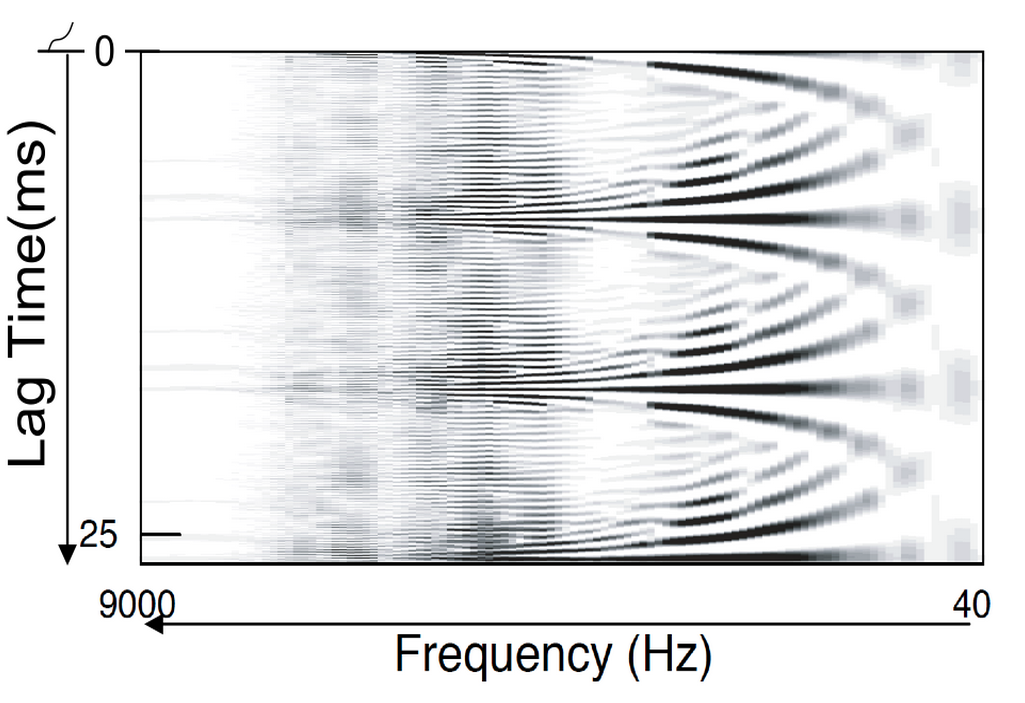
\includegraphics[width=150mm]{images/sai}
\caption{Stabilized Auditory Image \label{fig:sai}}
\end{figure}

This SAI image representation generates a 2D image of each section of
samples from an audio file.  We then reduce this large amount of
information in two steps, first by cutting the image into overlapping
boxes and finding row and column residuals of these boxes, and then by
vector quantizing the resulting high dimensionality vector.  The
resulting spare vector is then histogrammed across the audio file, and
this histogram is then used as input to an SVM \cite{yh05} classifier\cite{chapelle2006}.


